\documentclass{article}
\usepackage{tikz}
\usetikzlibrary{intersections,positioning,calc,shapes.geometric}
\usetikzlibrary{ext.paths.arcto}

\begin{document}

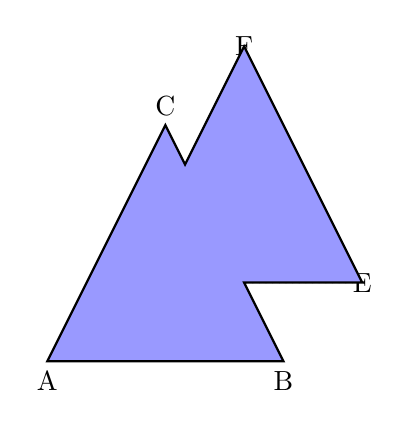
\begin{tikzpicture}

\coordinate (A) at (0,0);
\coordinate (B) at (3,0);
\coordinate (C) at (1.5,3);
\coordinate (D) at (1,1);
\coordinate (E) at (4,1);
\coordinate (F) at (2.5,4);

% Define the first triangle path
\path[dotted,name path=triangle1,draw] (A) node[below] {A} -- (B) node[below] {B} -- (C) node[above] {C} -- cycle;

% Define the second triangle path
\path[dotted,name path=triangle2,draw] (D) node {D} -- (E) node {E} -- (F) node {F} -- cycle;

% Define line segments as named paths
\path[name path=lineCB] (C) -- (B);
\path[name path=lineDF] (D) -- (F);
\path[name path=lineDE] (D) -- (E);

% Find intersections of lineCB with other lines
\path[name intersections={of=lineCB and lineDF, name=intCBDF}];
\path[name intersections={of=lineCB and lineDE, name=intCBDE}];

% % Place a node at the first intersection point
% \node[circle,fill=red,inner sep=2pt] at (intCBDF-1) {};
% \node[circle,fill=red,inner sep=2pt] at (intCBDE-1) {};

\filldraw[blue!40,draw=black,thick] (A) -- (B) -- (intCBDE-1) -- (E) -- (F) -- (intCBDF-1) -- (C) -- cycle;

\end{tikzpicture}

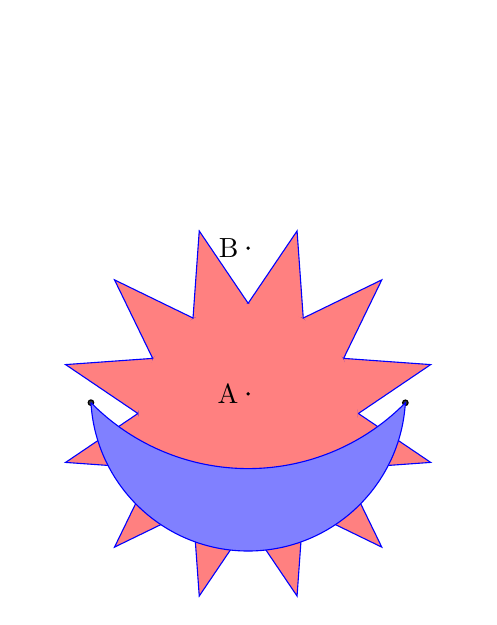
\begin{tikzpicture}

\coordinate (W) at (0:0);

\def\teeth{12}
\def\innerR{1.4}
\def\outerR{2.4}
\pgfmathsetmacro\angle{360/\teeth)}

\draw[blue,fill=red!50] (W) circle [radius=\innerR];
\draw[blue,fill=red!50]
  \foreach \i in {1,2,...,\teeth} {%
     [rotate=(\i-1)*\angle]  ($(W) + (0:\innerR)$) -- ($(W) + (\angle*1/2:\outerR)$) -- ($(W) + (\angle:\innerR)$)
   };
   
\pgfmathsetmacro\radA{2.0}
\pgfmathsetmacro\radB{2.8}

\coordinate[label=left:A] (A) at (0, 0.25);
\coordinate[label=left:B] (B) at (0, 2.1);

\path[name path=CA] (A) circle (\radA);
\path[name path=CB] (B) circle (\radB);

\foreach \i in {A,B} {
  \filldraw[black] (\i) circle (0.4pt);
}

\path[name intersections={of=CA and CB, by={I1,I2}}];

\draw[fill=black!80] (I1) circle (1pt);
\draw[fill=black!80] (I2) circle (1pt);

% \draw[blue,fill=blue!50] (I1) arc to[radius=\radB,large,clockwise](I2)
% arc to[radius=\radA,large](I1) ;
\draw[blue,fill=blue!50] (I1) arc to[radius=\radA](I2)
arc to[radius=\radB,clockwise](I1) ;

\end{tikzpicture}

\end{document}
